
                    \documentclass[a4paper, 12pt]{article}
                  \usepackage[english]{babel}
                  \usepackage[utf8]{inputenc}
    		\usepackage[utf8]{inputenc}
    %                \renewcommand{\baselinestretch}{1.0} 
                    
                    
                    %MARGINS
                    \usepackage[left=25.4mm, right = 25.4mm, top=25.4mm, bottom=25.4mm, includefoot]{geometry}
      %            \geometry{a4paper, total={170mm,257mm}, left=25.4mm, right = 25.4mm, top=25.4mm, bottom=25.4mm}
                    \setlength{\parindent}{0in}
                    \usepackage{enumitem}
                   
                    %Adding pictures
                    \usepackage{graphicx}
                    \usepackage{float}
                    
                    %Header and footers
                    \usepackage{fancyhdr}
                    \pagestyle{fancy}
%                    \fancyhead{}
                    \fancyfoot{}
                    \fancyfoot[R]{ \thepage\ }
                    \renewcommand{\headrulewidth}{0pt} %change the pt width to insert header line
                    \renewcommand{\footrulewidth}{0pt} %change the pt width to insert footer line
                    \usepackage{amsmath}
                    \fancyhf{}
                    
%    	\rhead{\leftmark}
%    	\lhead{Guides and tutorials}
	\rfoot{Centre for Civil Society \hspace{1mm} \textbar \hspace{1mm} www.ccs.in \hspace{2mm}  \thepage}
%             \lfoot{  \leftmark }     			% get the section heading on the footer 
                   
                   
                    %Tables
                    \usepackage{booktabs}
                    \usepackage{subfig}
                    \captionsetup{aboveskip=14pt,}
                    
                    %Coloured Boxes
                    \usepackage{xcolor}
                    \usepackage{mdframed}
                    
                    %Custom Spacing
                    \usepackage{setspace}
                    
                    %Defining Colours
             \definecolor{CCSbrown}{RGB}{163, 86, 37}
               \definecolor{CCSgrey}{RGB}{167, 169, 172}
                 \definecolor{CCSblack}{RGB}{64, 64, 65} 
             
             
             %Heading colours                  
                    \usepackage{sectsty}
                    \usepackage{titlesec}
    		\chapterfont{\color{blue}}  % sets colour of chapters font
    		\sectionfont{\color{CCSbrown}}  %sets colour of section font
    		\subsectionfont{\color{CCSblack}} %sets colour of subsection font
    		\subsubsectionfont{\color{CCSgrey}} %sets colour of subsubsection font
    		
		
		%Bibliography
		
		\usepackage[authordate, backend=biber]{biblatex-chicago}
		\addbibresource{universalrefs.bib}
		
		%
         
                    \begin{document}
                    
    %==================================================                
                    %TITLE PAGE
                    \begin{titlepage}
                    	\begin{center}
                    	\line(1,0){300}\\
                    	[0.25in]
                    	\huge{\bfseries \textcolor{CCSbrown} {Extracting E-fficiency}} \\
    	[0.5cm]
    	\large  {Making Extended Producer Responsibility \\ Work for E-Waste in India} \\
    	
                    	\line(1,0){200}\\
                    	[1in]
                    	\textsc{\huge Tarini Sudhakar, Akshat Singh,\\ Shubham Singh} \\
                    	[1.5cm]
                    	{\Large September 2018} \\
                    	[2.0cm]
    %    	{\huge Researching Reality Internship 2018} \\
     %   	[0.5cm]
                    	{\LARGE Centre for Civil Society} \\
                    	[0.1mm]
                    	{\Large New Delhi, India} \\
    	[2.0cm]
    	 
\includegraphics[width = 75mm]{CCSlogo.jpg}
      
                    	\end{center}
                    \end{titlepage}
     %=====================TOC===============================================                 
                    \tableofcontents
                    
     %======================LIST OF ABBREVIATIONS================================         
                   \newpage
                   \newlist{abbrv}{itemize}{1}
        \setlist[abbrv,1]{label=,labelwidth=1in,align=parleft,itemsep=0.1\baselineskip,leftmargin=!}
         
        \section*{List of Abbreviations}
        \addcontentsline{toc}{section}{List of Abbreviations}
        
        %\chaptermark{List of Abbreviations}
         
        \begin{abbrv}
         
        \item[CPCB]			Central Pollution Control Board
        \item[CTE]				Consent to Establish
        \item[CTO]			Consent to Operate
        \item[DIC]				District Industries Centre
        \item[DRS]			Deposit Refund Scheme
        \item[EEE]				Electronics and Electrical Equipment 
        \item[EPR]				Extended Producer Responsibility 
        \item[EWM]			E-Waste Management
        \item[HWM]			Hazardous Waste Management
        \item[HOWM]			Hazardous (and Other Wastes) Management
        \item[MoEFCC]			Ministry of Environment, Forest, and Climate Change
        \item[MTA]				Metric Tonnes per Annum
        \item[NCR]			National Capital Region
        \item[PET]				Polyethylene Terephthalate
        \item[PCC]			Pollution Control Committee
        \item[PRO]			Producer Responsibility Organisation
        \item[SPCB]			State Pollution Control Board
        \item[TSDF]			Treatment, Disposal, and Storage Facility
        \item[UP]				Uttar Pradesh
        
        
         
        \end{abbrv}
        
                    
                    %EXECUTIVE SUMMARY
                    \newpage
                    \section*{Executive Summary}
                    \addcontentsline{toc}{section}{Executive Summary}
                    India generates 2 million metric tonnes of e-waste annually and ranks amongst the top five e-waste generating countries in the world. The informal sector handles almost 95\% of this amount in India \parencite{shleifer1993corruption} (ASSOCHAM 2018). Only 5\% of the total e-waste is recycled and over 90\% is processed informally (ASSOCHAM 2018; Kumar 2018). The formal recycling sector in India is still developing while the informal recycling operations have been in place for a long time, employing over one million people (Bald et al. 2017).  \\
                    
                    The profit in recycling e-waste lies in extracting and re-selling metals from the electronic products. While it is profitable to extract metals like gold and copper, the extraction of mercury and lead is not as financially rewarding (Worstall 2016). Moreover, the latter metals are also hazardous substances and need to be disposed of properly. \\
                    
                    Unfortunately, informal recyclers circumvent the cost of treating these toxic components by dumping them in the open. This neglect contaminates the soil and pollutes the water bodies.\\
                    
                    Government of India has attempted to divert the flow of e-waste from the informal sector to the formal sector through the Extended Producer Responsibility (EPR) model introduced in the E-Waste Management (EWM) Rules, 2011. Producers?defined in the EWM Rules as any people who manufacture or sell electrical and electronic equipment and their components?are obligated under EPR to channelise the e-waste generated by their products to authorised recyclers. They do so by collecting their products back from the consumers and selling the e-waste to the authorised recyclers.  \\
                    
                    However, this envisioned EPR model does not match with the actual flow of e-waste in India. Our interviews with authorised recyclers in India made us realise that many of the 178 formal recycling firms registered under the Central Pollution Control Board in 2016 are currently performing under-capacity or running losses while the informal sector controls a significant portion of the e-waste market. We found out that this is because the informal recyclers quote at least double the prices offered by the formal recyclers for processing e-waste. Through this study, we attempt to understand the factors that hinder the formal recycling sector from keeping up with the informal sector?s pace. 
                    The first section of the paper examines the EPR model in India and the changes brought forth by the EWM Rules, 2016 to cover the leakages to the informal sector. These adjustments include the introduction of collection mechanisms other than take-back schemes and collection centres. \\
                    
                    The second section compares the intended and actual flow of e-waste in India. The next section explores the possible reasons for this dissonance and the failure of the current EPR model. The key limitation is narrowed down to the prices offered by the informal recycler. We then study the operating costs for both informal and formal recyclers that cause a disparity in their respective prices for e-waste to manifest. These costs include the licences required to enter the formal recycling market, compliance with government regulations, secure disposal of hazardous residue, and secondary markets for refurbished goods. \\
                    
                    The last section lays out a proposal for a revitalised EPR model that tackles the price difference between informal and formal recyclers in India. Our model suggests three modifications to the existing EPR system in the form of a Mandatory Deposit Refund Scheme, a Common Deposit Account, and third-party audits. The audits check e-waste from moving into the informal sector, and the Mandatory Deposit Refund Scheme incentivises the consumers to return their devices to the producers and not the kabadiwala. The Common Deposit Account is a way to enhance the efficiency of the model. It collects all the Deposit Refund fees into a common account which allows the consumers to return their devices to any producer. \\
                    
                    %INTRODUCTION
                    \newpage
                    \section{Introduction}
                    TThe production of electronic appliances has been steadily rising over the years, and their demand does not see signs of waning anytime soon (Chidambaram, Samuel, and Needhidhasan 2014). India?s electronics and hardware industry is expected to grow at a CAGR of 12-13\% and reach \$112-133 billion by 2018 (EY-ASSOCHAM 2016). New producers from Brazil, India, and China and the widespread use of semiconductors have been instrumental in bringing down the cost of manufacturing electronic devices and hence, their prices (Ahmed 2016). \\
                    
                    The fall in prices alongside a growing middle class with increasing disposable income contributes to a larger market for electronics and electrical equipments (EEE) (Livemint 2018). Consumers are driven to replace functional products as soon as newer models enter the market (Ala-Kurikka 2015). Planned obsolescence has also increased the units of EEE sold to replace products from 3.5\% in 2004 to 8.3\% in 2012 (Ahmed 2016).\\
                    
                    This rise in the manufacturing of EEE has been simultaneously followed by an increase in the amount of e-waste or end-of-life EEE generated. The global volume of e-waste is expected to reach 52.2 million MTA (metric tonnes per annum) by 2021 at an annual growth rate of 3.15\% (ASSOCHAM 2018). \\
                    
                    E-Waste is a pertinent ecological issue. EEE include certain components that are made of valuable metals such as gold and copper. It is profitable to process these parts and re-sell the metals as raw material. However, electronic products also contain a mix of toxic elements like arsenic and lead. These hazardous constituents are often not recycled because it is deemed more economical to recycle the valuable metals and dispose of the rest (Worstall 2016). If disposed improperly, the toxic components can cause significant environmental damage. Harmful metals such as lead and mercury can contaminate the topsoil and leach into the groundwater. \\
                    
                    This is a classic market failure caused by negative externalities. The market is unable to ensure the proper treatment of these toxic non-recyclable parts. Therefore,  government interventions are necessary to safely dispose the hazardous residue. Accordingly, the Government of India has issued the E-Waste Management (EWM) Rules, 2016. As per these rules, E-Waste Management in India is under the ambit of the Ministry of Environment, Forest, and Climate Change (MoEFCC). The MoEFCC has mandated producers and recyclers to obtain an ?authorisation? under the EWM Rules, 2016, and Hazardous and Other Wastes (Management and Transboundary Movement) (HOWM) Rules, 2016. \footnote{Only applicable to those who process e-waste that comes under Part C, Schedule III of the HOWM Rules, 2016} Producers and recyclers are allowed to continue operations in India only if they meet necessary standards for the  safe and proper handling of e-waste.
                     
                    Despite these regulations, more than 95\% of the generated e-waste ends up with the informal sector, which operates without the necessary authorisations (ASSOCHAM 2018). Much of the informal recycling takes place through open burning, grinding and washing, and acid baths (CSE 2015). These processes are highly dangerous and release toxic elements into the environment. For instance, the informal recyclers in Moradabad, Uttar Pradesh sieve the leftover ash from burning e-waste through the Ramganga river to recover small copper bits (CSE 2015, 6). \\
                    
                    Informal recyclers further amplify the problem by dumping the non-recycled hazardous components openly on the riverside or the ground. Studies show that the soil in areas such as Loni, Mandoli, and Krishna Vihar is deeply contaminated with heavy metals (Toxics Link 2014; Saha 2018). Moreover, the informal workers also do not have the necessary tools for the safe handling and recycling of e-waste (Kumar 2018). This neglect leads to severe (individual and public) health repercussions (Bhowmick 2011). \\
                    
                    In order to divert the supply of e-waste to the formal sector, Government of India introduced the concept of Extended Producer Responsibility (EPR) to e-waste in India in 2011. The concept was adopted after it successfully solved similar problems in other countries. However, its implementation in India did not deliver the expected results. The informal sector still processes most of the e-waste in India. Therefore in this paper, we look at the concept of EPR, the design of the current model in India, examine its shortcomings, and propose improvements to cover its limitations. Our study is based on interviews with formal and informal recyclers operating in the National Capital Region (NCR) of India. 
                    
                    %Extended Producer Responsibility for E-Waste in India
                    \section{Extended Producer Responsibility for E-Waste in India}
                    
                    On April 8, 2010, a man was exposed to Cobalt 60 while attempting to dismantle radioactive pipes in Mayapuri?one of the informal e-recycling hubs in Delhi. He died 19 days later due to the adverse effects of the radiation. There were several other victims of the same (Bhaduri 2017). The outcry that followed pushed the government into passing the E-Waste Management Rules in 2011. \\
                    
                    While many environmental regulations were put in place in India for managing hazardous waste, until 2011, e-waste was only dealt with briefly under two laws?the Hazardous Waste Management (HWM) Rules, 2008 and the Batteries (Management and Handling) Rules, 2001. The government had not enacted any rules that were explicitly dedicated to e-waste. This patchwork of legislation was hampered without any effective enforcement of the existing regulations (Kumar and Singh 2013). For instance, the Hazardous Waste Management (HWM) Rules, 2008 required any person recycling or reprocessing hazardous waste, including e-waste, to acquire authorisation from the Central Pollution Control Board (CPCB). However, only 23 recyclers had been authorised under the HWM Rules till 2010 (Bhaskar and Turaga 2017). It was the informal sector that predominantly handled the supply of e-waste (Thakur 2017). \\
                    
                    The consumer would sell the products to the kabadiwala once the EEE had completed their lifespan. The kabadiwala then resold the collected waste to the local scrap dealers. The scrap dealers sorted the waste, and sold it to the informal dismantlers, refurbishers and recyclers. \\
                    
                    Falling under the jurisdiction of the MoEFCC, the EWM Rules, 2011 defined electronic waste or e-waste as ?electrical and electronic equipment that has been discarded in whole or in part by individual and bulk consumers and during manufacturing, refurbishment, and repairing processes? and introduced the concept of Extended Producer Responsibility. \\
                    
                    \subsection{Concept of Extended Producer Responsibility}
                    
                    Extended Producer Responsibility holds the producer physically or financially responsible for the total environmental damage caused by his/her product at the end of its lifespan (Walls 2004). Thomas Lindhqvist, a Swedish academic, introduced the concept of EPR to the Government of Sweden in 1990. It was then implemented for the first time in 1991 in Germany to manage the waste generated by the packaging industry (Toxics Link 2007).\\
                    
                    When EPR is implemented in a sector, the producer?s responsibility is extended from the product?s manufacturing and consumption to its treatment at the end of its life (Toxics Link 2007). For example, consider the implementation of EPR in the bottled water sector. In a world without EPR, a company selling bottled water in polyethylene terephthalate (PET) bottles would only be responsible for the quality of the bottle and the water within. Despite the pollution risk posed by the PET bottle, neither the  company nor the consumer would be liable for its safe disposal. With EPR, the company would not only be responsible for the water and its packaging, but also for ensuring the secure disposal of PET bottles after usage. \\
                    
                    In traditional waste management models, consumers bear the burden of ensuring proper waste disposal. The local administration taxes consumers, and the revenue generated is used to run a waste management system. Nonetheless, this system does not incentivise the producer to reduce the negative environmental externalities caused by their products. EPR changes this incentive structure and holds the producers responsible for the inflicted environmental harm (Bhaskar 2011). \\
                    
                    \subsection{Current Design of EPR for E-Waste in India}
                    
                    With the objective to divert the e-waste from the informal sector and ensure its safe disposal, the EWM Rules, 2011 introduced EPR to waste management in India. It made the producers of EEE responsible for collecting the e-waste and ensuring its safe disposal. 
                    However, the rules failed to achieve the anticipated results. While the formal recycling capacities may have increased, the formal recyclers still received only 5\% to 15\% of the total supply of e-waste. Instead of encouraging the development of better collection and recycling infrastructure, the EWM Rules of 2011 ended up compelling the producers to implement a few inexpensive aspects of EPR (Bhaskar and Turaga 2017). \\
                    
                    Therefore, to fix these shortcomings, the EWM Rules 2016 were implemented. The three significant changes under the new rules were the modification of the existing EPR Authorisation process, the addition of various collection mechanisms for the producers to comply with EPR, and the institution of mandatory collection targets. If the producers defaulted on any of these counts, they could be charged a fine of Rs. 1 lakh or serve a jail sentence of five years under per the Environmental Protection Act, 1986. \\
                    
                    \subsubsection{EPR Authorisation}
                    
                    EPR Authorisation ensures that producers can be held accountable for channelling their e-waste to authorised recyclers. The authorisation requires a detailed EPR Plan outlining the producer?s chosen mechanism for EPR implementation and agreements with authorised dismantlers and recyclers. It also helps the government maintain a record of all the firms processing e-waste in the country. As per Rule 13 (1) (iv) of the EWM Rules, 2016, if the producers? applications for EPR Authorisation fail, their operations will cease to function until they are duly authorised to exercise EPR.\\
                     
                    There was significant delay in receiving the Authorisations from the state bodies under the EWM Rules, 2011. This caused further postponement of EPR implementation in India. Therefore, in 2016, CPCB took the responsibility for granting EPR-Authorisation in order to speed up the authorisation process (PIB 2016). \\
                    
                    \subsubsection{Collection Mechanisms}
                    
                    EWM Rules, 2011 had failed to mention any specific method apart from setting up collection centres and imposing take-back arrangements for implementing EPR. This ambiguity contributed to the difficulty of its execution (PIB 2016). For example, a study undertaken in 2015 showed that almost 35\% of the major EEE (both international and domestic) producers in India had either taken zero or limited action to implement EPR. Another 29\% had attempted to set up mechanisms but failed to achieve positive results. Most of these producers neither established take-back systems nor conveyed information about e-waste to their consumers as directed in the EWM Rules, 2011 (Toxic Links 2015).\\
                    
                    Therefore, to make it easier for the producers to implement their EPR, EWM Rules of 2016 offered new instruments for channelising the e-waste towards authorised recycling and disposal. These included the Deposit Refund Scheme (DRS) and Producer Responsibility Organisations (PROs). \\
                    
                    \paragraph{Collection Centres}
                    
                    According to the EWM Rules, 2011, collection centres refers to collection points or centres established to gather e-waste. The centres had to acquire authorisation from the SPCBs to operate. The EWM Rules, 2016 removed the need for this authorisation to allow flexibility for the producers while executing their EPR (PIB 2016). They could now be set up by an individual producer or an association, PROs, dismantlers, recyclers in order to channel waste to the authorised recyclers (PIB 2016).\\
                    
                    \paragraph{Deposit Refund Scheme}
                    
                    The Deposit Refund Scheme taxes the consumption of a product with a rebate on the return of the product or its packaging after usage (Walls 2011). The EPR-authorised producers charge a refundable fee from the consumers at the time of purchase. The consumers receive this fee back only when they deposit the products at the end of its life with the producers. Therefore, the deposit incentivises the consumers to return the used products to the producers. \\
                    
                    \paragraph{Producer Responsibility Organisation}
                    
                    Producer Responsibility Organisations (PROs) serve as a means for the producers to outsource their EPR implementation to meet collection targets. PROs aid producers by setting up and running collection centres, spreading awareness about e-waste to consumers and can also enact mechanisms such as a take-back or a Deposit Refund Scheme (CPCB 2018).\\
                    EWM Rules, 2016 recognise PROs as an important stakeholder in the e-waste market in India. Given their steadily growing presence, PROs are now also required to register with the CPCB as per Rule 13 (1) (xvii) of the EWM Amendment Rules, 2018. Upon a failure to do so, the PROs would face penalisation under the Environmental Protection Act, 1986.\\
                    
                    \subsubsection{Mandatory Collection Targets}
                    
                    EWM Rules, 2016 also sought to improve the success rate of EPR implementation by introducing mandatory minimum collection targets for each producer (PIB 2016). The EPR collection target was set as 30\% of the quantity of waste generated by the producers for 2016-2018. This target would increase in the subsequent years, and by 2022, the producers would have to collect 70\% of the waste generated.\\
                    However, in March 2018, the MoEFCC amended the EWM Rules, 2016 and reduced the collection targets. Producers were required to collect only 10\% of the e-waste generated in 2017-18 with 10\% annual increments. After 2022, they would need to meet the EWM Rules target of 70\% waste generated. This mandated rate is significantly higher compared to the collection rates in many developed countries which plateau between 40-50\% (SAGIS EPR 2014).  \\
                    
                    The amendment also introduced separate EPR targets for newer producers. As per Rule 13 (1) (xii) in the EWM Amendment Rules of 2018, these new producers were defined as those who had been operating in the market for a shorter period than their product?s average lifespan. Their EPR collection targets were based on the previous year?s sales figures and were lower than the targets for the older producers. \\
                    
                    
                    %Movement of E-Waste after EPR
                    
                    \section{Movement of E-Waste after EPR}
                    
                    The EWM Rules, 2016 made significant changes to the EPR model in order to divert the supply of e-waste to the formal recyclers. However, the actual movement of e-waste continues to differ significantly from the intended direction as the informal sector still handles more than 95\% of the domestically generated e-waste (ASSOCHAM 2018).\\
                    
                    
                    \subsection{Intended Flow of E-Waste}
                    
                    The mechanism envisioned in the EWM Rules, 2016 (see Fig. 1) to reroute the flow of e-waste to the formal recyclers involved four key steps:\\
                    
                    \begin{enumerate}
                      \item After using the EEE, the consumers would deposit the product (e-waste) with the authorised producers.
                      \item Mandated targets would compel producers to collect the e-waste by employing one (or a combination) of the several collection mechanisms. 
                      \item The producers would channel the collected e-waste to authorised recyclers.
                      \item The recyclers would then choose to either recycle or refurbish the e-waste and send the hazardous residue to Treatment, Storage and Disposal Facilities (TSDFs).
                    \end{enumerate}
                    
                    The government would place two checks to ensure that the objective of EPR is fulfilled. First, it would monitor the producers to ensure that they meet the annual collection targets. Second, it would audit the authorised recyclers to ensure that they dispose of hazardous material safely.\\
                    
                    %Figure 1
                    \begin{figure}[H]
                    	\centering
                    	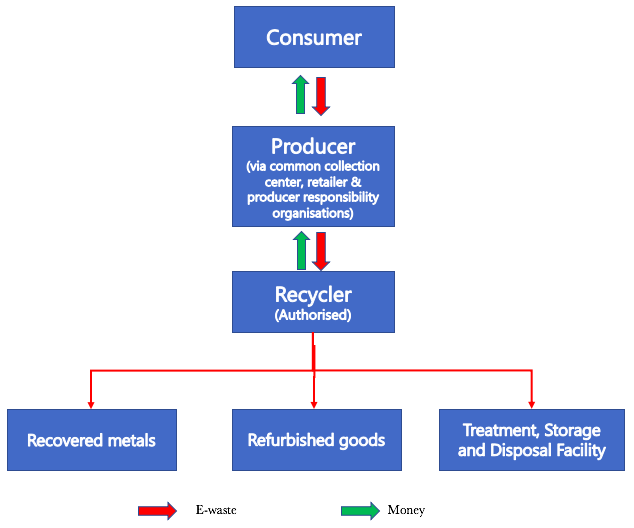
\includegraphics[height = 3in]{/Users/Alston/Documents/CCS/MSME/Latex/E-waste/fig1.png}
                    	\caption[Optional Caption]{EPR Model in India as per EWM Rules, 2016}
                    \end{figure}
                    
                    \subsection{Actual Flow of E-Waste}
                    
                    In reality, the flow of e-waste in India is much more complicated. Based on our interaction with formal and informal recyclers, we realised that the EPR model visualised in the EWM Rules, 2016 was not functioning as intended. \\
                    
                    For instance, NCR generates 85,000 metric tonnes of e-waste annually and has 28 recycling firms with a capacity of 1,07,976 MTA (ASSOCHAM 2018). However, our survey of six recycling firms in Faridabad, Rohtak, Manesar, and Hapur showed that these formal recyclers were operating at 39.9\% of their total capacity (see Appendix I). Their capacity to process e-waste was far greater than the amount that they were recycling. \\
                    
                    Instead, most of the e-waste was diverted to the informal recyclers in the following manner.\\
                    
                    \begin{enumerate}
                      \item After using the EEE, the individual consumers sell the product (e-waste) to the kabadiwala instead of the authorised collection entities. The kabadiwala resells the waste to the informal recycler who processes it unsafely. 
                      \item The authorised producers meet their mandated targets by collecting their e-waste from bulk consumers like IT companies. It is more economical to meet a 10\% collection target by focusing on the bulk consumers than implementing any of the collection mechanisms specified in the Rules, 2016.
                      \item Producers sell this e-waste to the authorised recyclers. However, authorised recyclers do not process the e-waste.  
                      \item Instead, the authorised recycler sells the e-waste to the informal recyclers. These informal recyclers, after processing the waste, continue to dump the hazardous residue improperly.
                    \end{enumerate}
                    
                    The checks placed by the government have proven to be ineffective. In our interviews with the formal recyclers, we noted that some authorised producers and recyclers sold the e-waste that they had collected to the informal recyclers. \\
                    
                    Our visit to Seelampur corroborated this circumvention of regulations. We posed as potential consumers looking to sell e-waste and asked if we could have some legitimate proof of our transaction. In response, the informal recycler offered us a certificate that verified his status as an authorised recycler and a GST transaction ID validating our sale. In this manner, the formal sector diverted e-waste towards the informal recyclers. \\
                    
                    We argue that in reality, e-waste in India moves along the channels shown in Figure 2. \\
                    
                    %Figure 2
                    \begin{figure}[H]
                    	\centering
                    	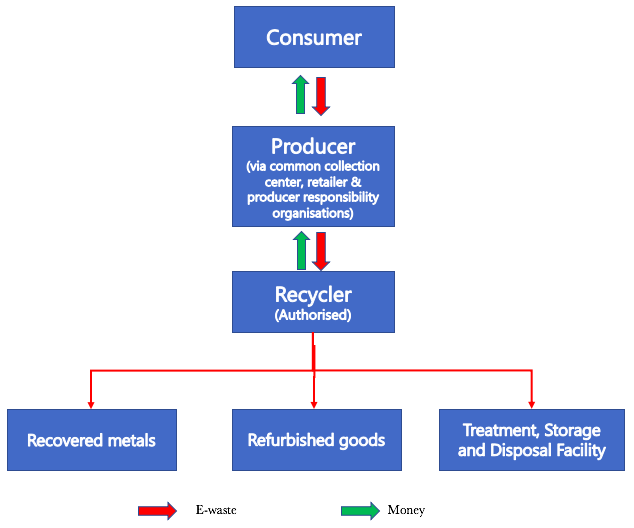
\includegraphics[height = 3in]{/Users/Alston/Documents/CCS/MSME/Latex/E-waste/fig1.png}
                    	\caption[Optional Caption]{EPR Model in India as per EWM Rules, 2016}
                    \end{figure}
                    
                    %Price Difference Between Informal and Formal Recyclers
                    \section{Price Difference Between Informal and Formal Recyclers}
                    
                    To understand why consumers were routing e-waste to the informal recyclers, we visited some of the e-waste hubs of Delhi?namely, Seelampur and Shastri Park. We averaged the prices offered for end-of-life EEE by seven informal shops in Shastri Park and Seelampur and five formal recycling firms spread across NCR (Faridabad, Hapur, Panipat).\\
                    
                    Table 1 lists the prices offered by the informal and formal recyclers for the most common EEE. \\
                    
                    
                    % Table generated by Excel2LaTeX from sheet 'Sheet1'
                    \begin{table}[htbp]
                      \centering
                      \caption{Price Comparison between the Informal and Formal Recycling Sectors}
                        \begin{tabular}{lrr}
                        Item  & \multicolumn{1}{p{8em}}{Informal Recycler \newline{}(Rs. per unit)} & \multicolumn{1}{p{8em}}{Formal Recycler \newline{}(Rs. per unit)} \\
                        \midrule
                        Toshiba Hard Disk (500GB/1TB) & 221.3 & 28.6 \\
                        CRT TV (Colour) & 325   & 127.5 \\
                        LCD TV (32-40 inches)r & 1642.9 & 403.3 \\
                        LED TV (32-40 inches) & 2107.1 & 436.6 \\
                        Air Conditioner (AC) (1.5 ton) & 2835.7 & 2058.3 \\
                        Computer Monitor (15-17 inches) & 371.4 & 302.6 \\
                        HP CPU (500 GB 16 GB RAM) & 2253.6 & 351.6 \\
                        Samsung Mobile S6 & 1418.6 & 62.5 \\
                        HP Laptop (i3/i5) & 4642.9 & 1133.3 \\
                        Refrigerator (350 litres) & 3514.3 & 683.3 \\
                        Printer (HP 1010) & 828.6 & 75.8 \\
                        UPS/Stabiliser  & 324.3 & 112.5 \\
                        Fax Machine  & 197.9 & 40 \\
                        \end{tabular}%
                      \label{tab:addlabel}%
                    \end{table}%
                    
                    The informal recyclers quoted at least double the price of formal recyclers. ACs and computer monitors were exceptions; the prices given by both were almost similar as copper is the only metal that can be extracted from these devices at a profit. But this price difference (see Fig. 3) allowed the informal recyclers to attract more e-waste than the formal recyclers. \\
                    
                    %figure 3
                    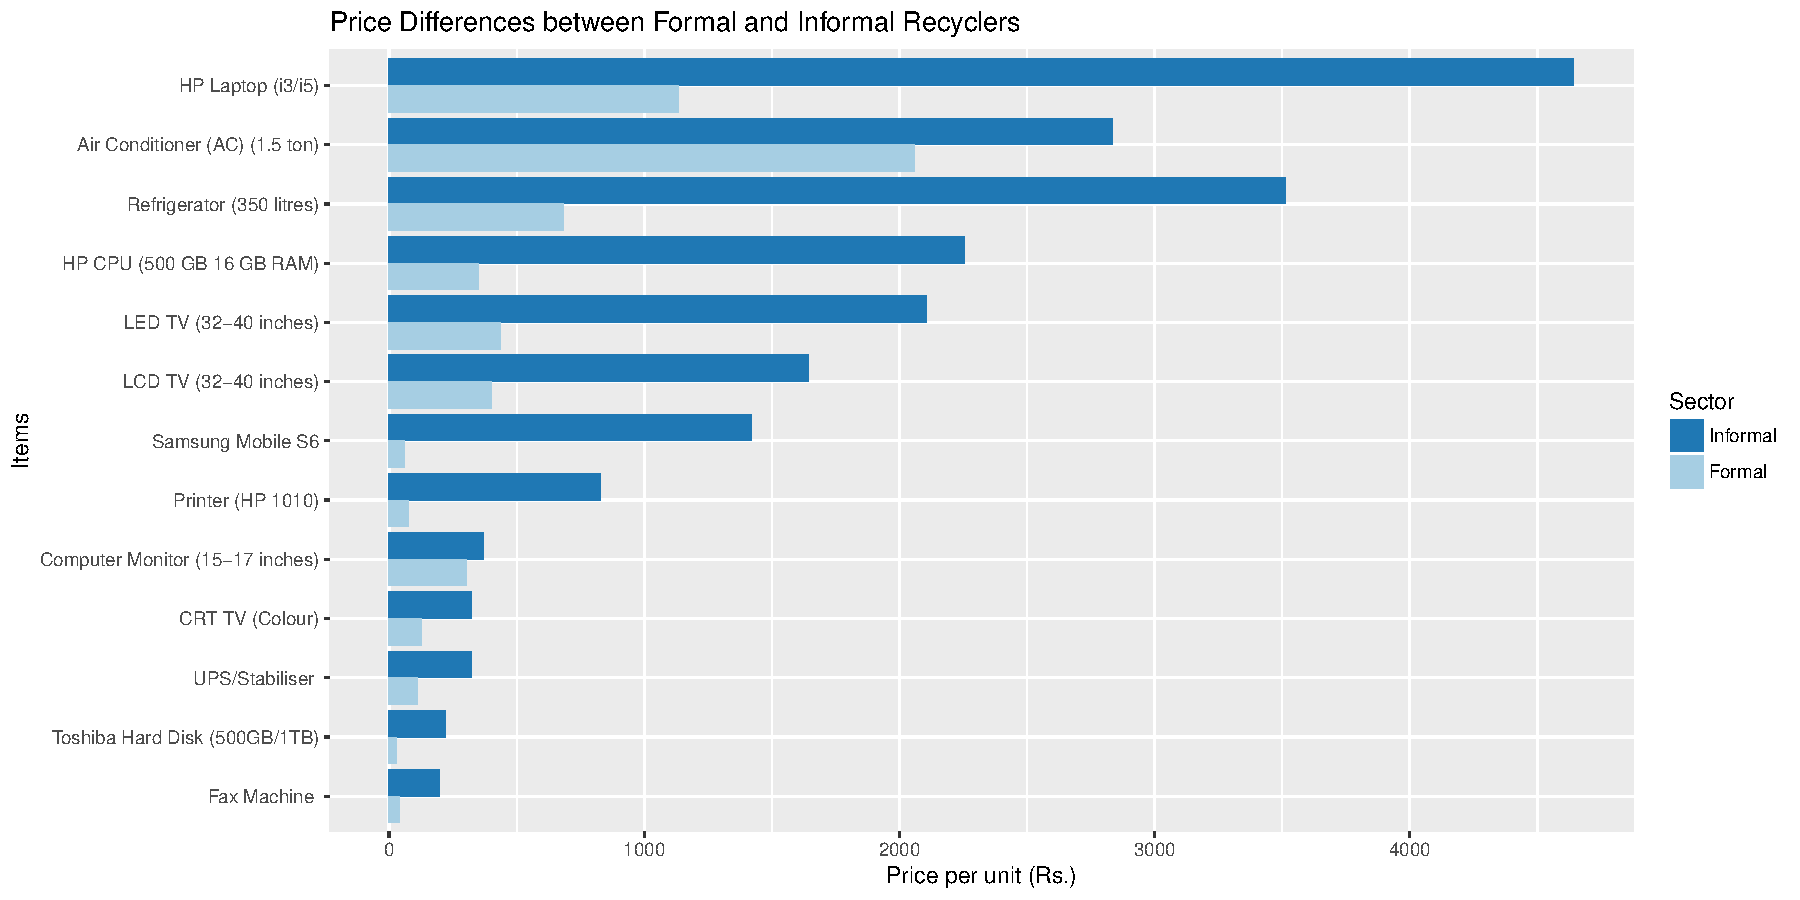
\includegraphics[width=0.98\textwidth]{myfile}
                    
                    
                    \subsection{Explaining the Price Difference}
                    
                    Informal recyclers function with far lower operating costs than the formal recyclers in India. These costs allow them to quote higher prices and capture a significant portion of the market (Chintan Environmental Research and Action Group 2013). In this section, we offer explanations accounting for the price difference between the informal and formal recyclers. \\
                    
                    \subsubsection{Cost of Licences}
                    
                    Under the EWM Rules, 2016, a recycler needs to acquire certain licences to begin operations. We hypothesised that the cost of acquiring these licences was significant, and would ultimately reflect in the price that the authorised recyclers could afford to pay for the e-waste. The informal recyclers do not bear this cost as they operate without the necessary licences. \\
                    
                    The formal recycler needs to acquire the following registrations/licences to start processing e-waste:\\
                    \begin{enumerate}
                      \item Consent to Establish (CTE) from the State Pollution Control Board (SPCB)
                      \item Consent to Operate (CTO) from SPCB
                      \item Certificate of Registration from District Industries Centre (DIC)
                      \item Proof of Installed Capacity of plant and machinery from DIC
                      \item Environmental Clearance from SPCB 
                      \item E-Waste Licence under the EWM Rules, 2016 from SPCB
                      \item Hazardous Waste Licence under the HOWM Rules, 2016 from SPCB. 
                    \end{enumerate}
                    
                    As the Environmental Clearance (no. 5) was required for plants with a capacity greater than 25000 MTA, and only 2 of the 178 registered plants had this capacity, its cost has been omitted from our calculations (CPCB 2016). The cost of registering with the DIC (no. 3 and no. 4) is also not included due to logistical restraints. \\
                    
                    The official costs for the E-Waste and Hazardous Waste licences comprise the cost of acquiring standard industry licences?CTE and CTO (no. 1 and no. 2). The official costs for these licences vary according to the firm?s initial investment. Through our interviews, we gauged this initial investment for a recycling firm to be between Rs. 1 to 5 crores. We then computed the official costs levied by each State Pollution Control Board for the industry licences using the information provided on the respective SPCB websites. \\
                    
                    As our study focuses on NCR, we specifically looked at the costs imposed by Uttar Pradesh (UP) and Haryana. We tried to capture the actual time taken to acquire the licences as it may have been a source of transaction costs, but we were only able to survey six firms in NCR. Therefore, we calculated the official time taken to grant licences in UP and Haryana. Table 2 records these costs. 
          
          %table2          
        % Table generated by Excel2LaTeX from sheet 'Sheet1'
        \begin{table}[htbp]
          \centering
          \caption{Official Cost of Acquiring CTE and CTO}
            \begin{tabular}{llll}
            \multicolumn{1}{p{5em}}{State} & \multicolumn{1}{p{5em}}{Licences} & \multicolumn{1}{p{12.585em}}{Cost in Rs. (for investment between 1 to 10 crores)} & \multicolumn{1}{p{7.165em}}{Official Time Taken (in days)} \\
            \midrule
            Uttar Pradesh  & CTE+CTO  & 117000 & 40-60 \\
            Haryana & CTE+CTO  & 384000 & 20-40 \\
            \end{tabular}%
          \label{tab:addlabel}%
        \end{table}%
                    
                    
                    
                    The official costs for these licences range between Rs. 1 to 4 lakhs. The average official time taken to obtain them is 1.3 months. According to our survey, the actual time taken to acquire these licences ranged from 20 to 60 months.\\
                    
                    \subsubsection{Cost of Regulatory Compliance}
                    
                    There are other regulations that the authorised recycler needs to comply with that the informal sector does not. Auditing and physical inspections are part of the scrutinisation process. These provisions place a check on the e-waste handled by the producers and recyclers and impose an additional cost on them. The informal recyclers do not incur these costs nor do they pay the appropriate taxes levied on authorised recyclers. \\
                    
                    There are also costs associated with adhering to labour regulations. An authorised recycler needs to implement specific occupational and safety measures before starting operations (see Appendix II). However, the informal recyclers often work with the bare minimum gear and do not comply with these rules. They also do not abide by child labour laws as over 4.5 lakhs children are allegedly employed by the informal sector (ASSOCHAM 2014).\\
                    
                    \subsubsection{Cost of Disposing Hazardous Residue }
                    
                    The formal recyclers incur additional costs when they attempt to meet the standards set by government regulations. However, even if these regulatory costs were lifted, the formal recyclers would still have to pay for safely disposing of the hazardous residue.\\
                     
                    The regulations in place to oversee the secure disposal of toxic components require authorised recyclers to send their processual residue to authorised Treatment, Storage, and Disposal Facilities. The unauthorised recyclers circumvent this obligation and avoid the cost of treating their toxic waste in TSDFs by dumping it in the open.\\
                    
                    \subsubsection{Access to Secondary Markets for Refurbished Goods}
                    
                    An often overlooked element of the e-waste market is the refurbishment and reuse of the waste EEE. More than recycling, the informal recycler focuses on reuse, resale, and refurbishment of goods (Gidwani and Corwin 2017). Much of e-waste is repaired and sold in secondary markets. These markets usually sell refurbished goods without obtaining prior approval from the producer companies. We also found out that Nehru Place and Gaffar Market are prime secondary markets in New Delhi. \\
                    
                    Reselling refurbished goods is more profitable than merely selling recycled metal. The unauthorised recyclers are at an advantage and can quote higher prices for the e-waste as the authorised recyclers are often forbidden from reselling. The producer companies that employ authorised recyclers to handle their e-waste fear the creation of parallel competition for their new products (Alev 2015). Our interviews with the authorised recyclers revealed that some of their clients (producer companies) demanded the recyclers to photograph the shredded e-waste. This evidence ensured that the recyclers could not resell the waste EEE in the secondary markets. \\
                    
                    There are numerous factors such as the ones mentioned above that contribute to the price gap between the informal and formal recyclers. This price gap incentivises the consumers to sell e-waste to the informal sector and thus, negates the envisioned EPR model. \\
                    
                    %Revitalised EPR Model
                    
                    \section{Revitalised EPR Model}
                    
                    In order to seal off the e-waste leakages to the informal market, the EPR model needs to tackle the difference in prices that formal and informal recyclers offer to buy e-waste. We suggest three modifications to the current system: a Mandatory Deposit Refund Scheme, Common Deposit Account, and third-party Audits. Audits are required to prevent e-waste from leaking to the informal sector, and the Mandatory Deposit Refund Scheme secures the supply of e-waste to the formal recyclers. The Common Deposit Account is an optional addition to improve the efficiency of the new model (see Fig. 4). \\
                    
                    \subsection{Mandatory Deposit Refund Scheme}
                    
                    Under the EWM Rules, 2016, producers can choose to execute their EPR through any scheme of their liking. Therefore, the decision to impose a Deposit Refund Scheme (DRS) lies with them. If a producer chooses to impose a DRS, it would increase the price of his product and reduce sales, making him less competitive in the market. Similar will be the case if any other collection mechanism is employed which directly imposes the cost on the producer. Therefore, it would be in the producer?s best interest to refrain from implementing it.\\
                    
                    When the Deposit Refund fee is made mandatory, all the authorised producers would be required to impose it. This would raise the prices quoted by all producers and decrease overall sales. However, no one producer would be singled out and be at a disadvantage.\\
                      
                    Unfortunately, the problem would persist if the producers are free to determine the quantum of the fee. It would be in their best interest to have the fee closest to zero, rendering the mandatory fees moot. Therefore, the minimum fee for every type of product should also be mandated. If this fee is higher than the price offered by the informal sector, the consumers will choose to sell their e-waste to the authorised producer as opposed to the kabadiwala. \\
                    
                    The government-mandated fee would also not entirely keep e-waste in the formal sector. Producers would still have an incentive to sell the waste to the informal sector as opposed to the authorised recyclers. Therefore, the third-party audits should cross-validate the Deposit Refund fees withdrawn from the producers? accounts to give the consumers against the e-waste sold to the authorised recyclers. \\
                    
                    Deposit Refund Schemes have been shown to improve recycling rates. For example, 44 states in the USA have implemented some variation of a DRS for lead-acid batteries. Retailers charge a \$10 deposit on batteries which is refunded to consumers if they return used batteries within 30-45 days of purchase. After the introduction of the DRS, the recycling rate for lead-acid batteries rose from 86\% to 97\% (Walls 2011).\\
                    
                    \subsection{Common Deposit Account}
                    
                    If a Deposit Refund Scheme is implemented either in the current or the proposed model, consumers would be unable to avail the Deposit Refund fee from a new producer who is different from the original producer. This is  because the Deposit Refund fee, initially deposited with the original producer, would be inaccessible to the new producer. \\
                    
                    A Common Deposit Account would solve this problem. If all the collected Deposit Refund fees were placed in an account accessible to all the producers, consumers would be able to receive their refund from any producer after depositing the end-of-life EEE. \\
                    
                    While there aren?t any large-scale applications of a Common Deposit Account for producers, countries have utilised common money funds to subsidise recycling. For instance, the Environmental Protection Administration (EPA) of the Government of Taiwan manages a Recycling Fund Management Committee (RFMC). Manufacturers and importers of EEE have to give funds into the Recycling Fund. These funds are used to provide subsidies for those participating in collection and recycling of e-waste (Chung, Murakami-Suzuki, and Kojima 2009). \\
                    
                    Therefore, in our model, the government would need to set up the Common Deposit Account and supervise the collection of all Deposit Refund fees received by producers. \\
                    
                    \subsection{Third-Party Audits}
                    
                    In the current system, the responsibility of safely disposing of the hazardous material lies with the authorised recyclers. However, the mechanism to oversee the execution of this responsibility is ineffective. As a result, some authorised recyclers sell the e-waste that they acquire to the informal sector for higher profit margins.\\
                    
                    A check should be established on the activities of the authorised recyclers to ensure that they properly treat the toxic content in the e-waste. The quantity of hazardous material in the e-waste transferred from the producer should be cross-validated against the quantity that the recyclers disposed of securely. While the government can audit the firms, past experience has proved it to be ineffective. Authorised producers and recyclers still sell their e-waste to the informal recyclers as mentioned earlier.\\
                     
                    An alternative would be to engage third-party auditors to perform the inspection processes.\\
                    
                     
                    %Figure 4
                    \begin{figure}[H]
                    	\centering
                    	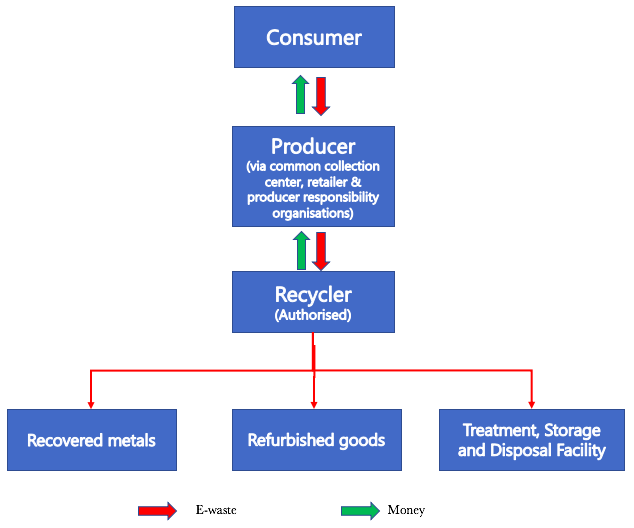
\includegraphics[height = 3in]{/Users/Alston/Documents/CCS/MSME/Latex/E-waste/fig1.png}
                    	\caption[Optional Caption]{EPR Model in India as per EWM Rules, 2016}
                    \end{figure}
                    
                    \subsection{Possible Repercussions}
                    
                    The implementation of the proposed EPR model may also have certain unfavourable consequences. It could lead to an increase in smuggled devices as the mandatory fees would be applicable only in India and would raise the prices of domestic products. Each producer could also potentially lose consumers who will look for cheaper alternatives.\\
                    
                    %Conclusion
                    
                    \section{Conclusion}
                    
                    The quantity of e-waste generated in Delhi-NCR is projected to hit 1,50,000 MTA by 2020 (ASSOCHAM 2018). Its potential for environmental and health hazards makes e-waste a critical issue to be dealt with.\\
                     
                    While the Extended Producer Responsibility model was a step in the right direction, it is yet to fulfil its aim. The informal sector processes over 95\% of e-waste in India often handling it roughly without the appropriate safety measures (ASSOCHAM 2018). Moreover, it dumps the toxic residue without treating it properly. \\
                    
                    In this paper, we studied the current EPR model to account for its limitations and focused on the sharp difference in prices offered by the informal and formal recyclers. Incentivised by these higher prices of the kabadiwala or the local scrap dealer, consumers sold their products to the informal sector instead of returning the EEE to the producers. \\
                    
                    Our proposed modifications to the existing EPR model would tackle this price gap in three ways. The Deposit fee equalling or higher than the informal sector?s prices would keep the consumers from selling their products to the kabadiwala and the Common Deposit Account would make it convenient for the consumers to return their devices to the producers. The third-party audits would cross-check the amount of e-waste transferred from the producers with the quantity processed by the authorised recyclers. This would help ensure that the hazardous residue is treated properly.\\
                    
                    This is only a broad idea of how the EPR model can be reformed. Further research needs to be conducted to hammer out the execution. Aspects such as incentivising the reduction of hazardous substances in EEE and interest rate on the Deposit Refund fees have to be taken into account. Moreover, it is difficult to gather information on the different types of EEE and set the optimal quantum of fees that will direct e-waste to the formal recyclers. Therefore, an alternate scenario where the market, instead of the government, can set at the Deposit fees needs to explored. \\
         
% Print Bibliography

	\printbibliography[title={Bibliography}]
         
         
        %Appendix1     
             \section*{Appendix 1: Capacity of Recycling Firms}
             \addcontentsline{toc}{section}{Appendix 1: Capacity of Recycling Firms }
         % Table generated by Excel2LaTeX from sheet 'Sheet1'
        \begin{table}[htbp]
          \centering
          \caption{Actual Working and Optimum Recycling Capacity of Surveyed Firms}
            \begin{tabular}{lrr}
            \multicolumn{1}{p{5em}}{Name of Recycling Firm} & \multicolumn{1}{p{5em}}{Optimum Capacity (in tonnes)} & \multicolumn{1}{p{7.915em}}{Capacity Utilised for 2017-18 (in tonnes)} \\
            \midrule
            SMS Enterprises, Pace City, Gurgaon & 360   & 8 \\
            Namo E-Waste Management, Faridabad & 5796  & 870 \\
            Earth Waste Management, Rohtak & 600   & 400 \\
            Greeniva Recycler, Hapur & 1500  & 700 \\
            Royal Faiz Recycling, Hapur  & 9000  & 6500 \\
            Hind Recycling, Hapur & 9000  & 2000 \\
            \midrule
            Total & 26256 & 10478 \\
            \end{tabular}%
          \label{tab:addlabel}%
        \end{table}%
        
             
        %Appendix 2  
        \newpage
             \section*{Appendix 2: Additional Requirements for Authorising Recyclers}
           \addcontentsline{toc}{section}{Appendix 2: Additional Requirements for Authorising Recyclers}
        
        \begin{mdframed}[backgroundcolor=gray!20]
        According to the Implementation Guidelines given by CPCB for the EWM Rules, 2016, a recycling facility needs to provide the following to the SPCB:
            \begin{enumerate}[noitemsep,nolistsep]
            
                       \item Details of air pollution control devices along with diagram and design scheme
                        \item Details of effluent treatment plants (ETP) installed in the unit along with diagram and design scheme 
                        \item Details of storage facility separate for raw material, segregated material, dismantled parts, Hazardous Waste, Bag Filter Residue/Floor Cleaning dust, ETP sludge, non recyclable/non removable components.
                             \item Membership and registration with Treatment, Storage, Disposal Facility operator authorised under Hazardous Waste (MH\&TM) Rules, 2008
                              \item Power of attorney/authority letter of signature to the applicant
                               \item Details of handling, dismantling/recycling/refurbishing provided at the facility for e-waste and hazardous waste 		                  
                               \begin{enumerate}[noitemsep,nolistsep]
                          	 	\item Should include adequate wastewater treatment facilities and air pollution control equipment 
                    	 		 \item Provide technology for data destruction 
                      		 \end{enumerate}
                       \item Copy of allotment letter from MCD with details of land and building plan \\
            \end{enumerate}
            
            Recyclers are also required to operate on a minimum of 500 sq metres if their capacity is 1 MT (metric ton) per day.\\
            
            Documents to be submitted for the Hazardous Waste (under the HOWM Rules, 2016) licence to the SPCB are:
        
        \begin{enumerate}[noitemsep,nolistsep]
        	\item Certificate authorising the Occupier (any person who has control over a factory that deals with hazardous and other wastes)
        	\item Nature and quantity of different wastes received annually from domestic sources or imports
        	\item Emergency Response Plan with procedures to be followed in an emergency such as a spillage or a fire
        	\item Details of the secured storage facility for hazardous wastes and their mode of disposal
        	\item Details of pollution control systems such as ETPs
        	\item Details of occupational health and safety measures
        	\item Process flow sheet showing equipment details, inputs (raw materials), and outputs (products, by-products, waste, emissions)
        	\item Details of end user of products or by-products
        	\item Proof of application given to the operator of Common Hazardous and Other Wastes Treatment, Storage, and Disposal Facility (CHWTSDF)
        
        \end{enumerate}
        
            \end{mdframed}
         
         
         %Appendix 3
             \newpage       
             \section*{Appendix 3: Questionnaire Administered to Formal Recyclers}
             \addcontentsline{toc}{section}{Appendix 3: Questionnaire Administered to Formal Recyclers}
                    \setstretch{0.5}
                    \begin{mdframed}[backgroundcolor=gray!20]
                    \begin{enumerate}[noitemsep,nolistsep]
                       \item General Information:
                          \begin{enumerate}[noitemsep]
                          	 \item Name of the firm
                    	  \item When was it established? (mm/yyyy)
                    	   \item Where is it located?
                       \end{enumerate}
                       \item When did you begin to acquire licences to register your firm? (mm/yyyy)
                       \item How long did it take to acquire all the licences necessary for registration?
                       \item Were you able to find clear guidelines for acquiring the licences on the State Pollution Control Board (SPCB) website? 
                       \item Did you pay consultants/brokers/lawyers/others to help with the registration process? 
                       \item How long did it take for you to acquire the E-Waste licence (under the EWM Rules, 2016)?
                       \item What were the official costs incurred to acquire the E-Waste licence?
                       \item How long did it take for you to acquire the Hazardous Waste licence (under the HOWM Rules, 2016)? 
                        \item What were the official costs incurred to acquire the Hazardous Waste licence? 
                        \item When did you start processing e-waste? (mm/yyyy) 
                        \item Who are your major sources of raw material?
                        \begin{enumerate}[noitemsep]
                          	 \item Local Kabadiwalas
                    	  \item Unauthorised Scrap Dealers
                    	   \item Bulk consumers like IT companies 
                    	    \item Individual households 
                    	  \item Authorised Collectors/Producer Responsibility Organisations 
                    	   \item Others: \_\_\_\_
                       \end{enumerate}
                        \item What is the maximum recycling capacity of your firm? (in MTA)
                        \item What was the actual working capacity of your firm in the previous year? (in MTA)
                        \item What is the quantity of e-waste that is projected to be recycled by you in 2018? (in MTA) 
                         \item Has your firm reached its break-even point?
                         \item How long did it take to reach the break-even point after beginning operations? 
             \end{enumerate}  
            \end{mdframed}
                    
                    
                    
                    
                    \end{document}